\documentclass[a4paper,10pt,twocolumn]{article}
\usepackage{amsmath, amsthm, amssymb}
\newtheorem{theorem}{قضیه}[section]
\newtheorem{lemma}{لم}
\usepackage{graphicx}
\usepackage{fancyhdr}
\usepackage{geometry}
% --- Two-column paper layout tweaks ---
\setlength{\columnsep}{0.7cm}          % space between the two columns
\geometry{top=2cm,bottom=2cm,left=1.7cm,right=1.7cm}  % typical paper-like margins
\usepackage{cancel}
\usepackage{listings}
\usepackage{xcolor}

\usepackage[hidelinks]{hyperref}
\hypersetup{
  unicode=true,
  bookmarks=true,
  bookmarksnumbered=true
}
\usepackage{xepersian}

\settextfont{XB Niloofar}
\setlatintextfont{Times New Roman}

\lstdefinestyle{mypython}{
    language=Python,
    basicstyle=\ttfamily\footnotesize,
    keywordstyle=\color{blue},
    commentstyle=\color{gray},
    stringstyle=\color{red},
    frame=single,
    breaklines=true
}
% تنظیمات صفحه
\geometry{top=3cm, bottom=3cm, left=3cm, right=3cm}
\renewcommand{\baselinestretch}{1.5}
\setlength{\parindent}{0pt}
\setlength{\parskip}{8pt}

% تنظیمات هدر و فوتر
\pagestyle{fancy}
\fancyhf{}
\rhead{\textbf{تلاش‌هایی برای پیدا کردن کران بالایی بهتر برای مسئله بندیت پیوسته و لیپ‌شیتز }}
\lhead{\textbf{صفحه \thepage}}
\cfoot{}

\begin{document}

% صفحه عنوان
\begin{titlepage}
    \begin{center}
        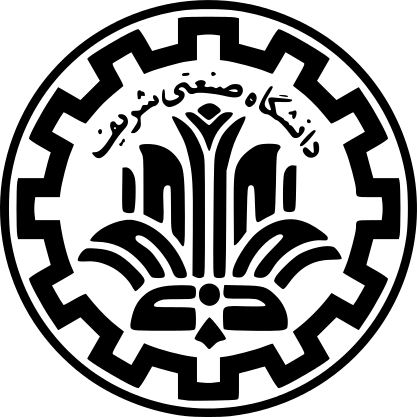
\includegraphics[width=0.2\textwidth]{Shariflogo.png} % تغییر دهید به مسیر لوگوی دانشگاه شما
        \\
        {\Huge\textbf{تلاش‌هایی برای پیدا کردن کران بالایی بهتر برای مسئله بندیت پیوسته و لیپ‌شیتز}}
        \\
        \rule{\linewidth}{1.5pt}
        \\
        {\Large \textbf{درس: آنالیز احتمالاتی ابعاد بالا}}
        \\
        \vfill
        {\Large \textbf{تهیه‌کنندگان:}}
        \\
        {\large مهدی دارابی} \\
        {\large حامی عبادزاده سمنانی} \\
        \vfill
        {\Large \textbf{استاد: دکتر محمدحسین یاسائی میبدی}}
        \\
        {\large دانشگاه صنعتی شریف}
        \\
        {\large \today}
    \end{center}
\end{titlepage}

\tableofcontents
\newpage

\begin{center}
    به نام خدا
\end{center}
\section{مقدمه}
\noindent
در بسیاری از مسائل تصمیم‌گیری، باید به‌صورت تکرارشونده یکی از چند گزینه را انتخاب کنیم، در حالی‌که کیفیت واقعی هر گزینه از پیش معلوم نیست و فقط با آزمون و مشاهده پیامدها آشکار می‌شود. مسئله‌ی \lr{Multi-Armed Bandit} یک چارچوب ساده برای مدل‌سازی همین وضعیت است و هسته‌ی اصلی آن «موازنه‌ی اکتشاف/بهره‌برداری» است: از یک سو باید گزینه‌های کمترشناخته را امتحان کرد تا اطلاعات به‌دست آید (اکتشاف)، و از سوی دیگر باید تا حد ممکن از گزینه‌ای استفاده کرد که تاکنون بهتر عمل کرده است (بهره‌برداری).

این چارچوب در کاربردهای متعددی ظاهر می‌شود؛ برای مثال در تبلیغات و \lr{A/B-test}، سامانه‌های پیشنهاددهنده، بهینه‌سازی برخط تجربه کاربری، و تخصیص منابع در شرایط عدم‌قطعیت. هدف، به‌طور کلی، بیشینه‌سازی عملکرد تجمعی در طول زمان است، در حالی‌که یادگیری نیز هم‌زمان با تصمیم‌گیری رخ می‌دهد. 


\section{تعریف مسئله (حالت گسسته و پاداش‌های کران‌دار)}
\label{sec:problem-definition}

\noindent
تعریف این بخش مطابق مقاله‌ی \lr{Auer, Cesa-Bianchi, and Fischer (2002)} است \cite{auer2002finite} و ممکن است در برخی منابع دیگر متفاوت ارائه شود.

\medskip

مسئله‌ی \lr{Multi-Armed Bandit} با $K$ بازو به‌صورت زیر مدل می‌شود.
برای هر بازو $i\in\{1,\dots,K\}$، دنباله‌ی پاداش‌ها
\[
Y_{i,1},Y_{i,2},\dots
\]
مستقل و هم‌توزیع با توزیع ناشناخته‌ی $P_i$ هستند و
\[
\mu_i \;:=\; \mathbb{E}[Y_{i,1}]
\]
امید پاداش بازوی $i$ را نشان می‌دهد.
همچنین دنباله‌های پاداشِ بازوهای مختلف نسبت به هم مستقل فرض می‌شوند.
در این مقاله پاداش‌ها کران‌دارند؛ یعنی برای هر $i$،
\[
\mathrm{supp}(P_i)\subseteq [0,1].
\]

یک سیاست یا \lr{Policy} در هر گام $t=1,2,\dots$ یک بازو را انتخاب می‌کند.
اگر $T_i(n)$ تعداد دفعات انتخاب بازوی $i$ تا پایان گام $n$ باشد، آنگاه پاداش تجمعیِ مورد انتظار برابر است با
\[
\mathbb{E}\!\left[\sum_{i=1}^K \sum_{s=1}^{T_i(n)} Y_{i,s}\right]
\;=\;
\sum_{i=1}^K \mu_i\,\mathbb{E}[T_i(n)].
\]

بازوی بهینه را با
\[
\mu^\ast \;:=\; \max_{1\le i\le K}\mu_i
\]
تعریف می‌کنیم. و در نهایت پشیمانی یا \lr{Regret} پس از $n$ گام برابر است با
\[
R(n)
\;:=\;
\mu^\ast n \;-\; \sum_{i=1}^K \mu_i\,\mathbb{E}[T_i(n)].
\]

\noindent
\textbf{هدف مسئله:} طراحی سیاستی که \lr{regret} را \emph{کمینه} کند؛ یعنی برای افق $n$ تا حد امکان مقدار $R(n)$ کوچک باشد.


\section{نمونه‌ای از سیاست‌های یادگیری در بندیت چند بازو}

\subsection{الگوریتم UCB1}

الگوریتم \lr{UCB1} که در \cite{auer2002finite} معرفی شده است،
برای هر بازو در هر گام یک «شاخص» تعریف می‌کند و بازویی را انتخاب می‌کند
که این شاخص بیشترین مقدار را داشته باشد.
اگر تا گام $t-1$، بازوی $i$ تعداد $T_i(t-1)$ بار انتخاب شده باشد،
میانگین تجربی آن برابر است با
\[
\widehat{\mu}_i(t-1)
=
\frac{1}{T_i(t-1)}
\sum_{s=1}^{T_i(t-1)} Y_{i,s}.
\]

در گام $t$ شاخص بازوی $i$ به‌صورت
\[
I_i(t)
=
\widehat{\mu}_i(t-1)
+
\sqrt{\frac{2\ln t}{T_i(t-1)}}
\]
تعریف می‌شود و بازویی انتخاب می‌شود که $I_i(t)$ را بیشینه کند.

جمله‌ی اول بیانگر برآورد فعلی کیفیت بازو (بهره‌برداری) و
جمله‌ی دوم بیانگر میزان عدم‌قطعیت نسبت به آن (اکتشاف) است.
هرچه بازویی کمتر آزموده شده باشد، جمله‌ی دوم بزرگ‌تر است و
الگوریتم آن را برای جمع‌آوری اطلاعات بیشتر ترجیح می‌دهد.
در آغاز اجرا، هر بازو یک‌بار انتخاب می‌شود تا میانگین تجربی آن تعریف گردد.

\subsection{کران پشیمانی سیاست UCB1}

\begin{theorem}
فرض کنید پاداش‌ها در بازه‌ی $[0,1]$ کران‌دار باشند.
اگر از الگوریتم \lr{UCB1} استفاده شود، آنگاه برای هر بازوی زیر‌بهینه
$i$ یعنی 
$\Delta_i := \mu^\ast - \mu_i > 0$،
تعداد انتخاب‌های مورد انتظار آن تا گام $n$ دارای کران زیر است:
\[
\mathbb{E}[T_i(n)]
\le
\frac{8 \ln n}{\Delta_i^2}
+ 1 + \frac{\pi^2}{3}.
\]

در نتیجه، پشیمانی کل دارای کران لگاریتمی زیر خواهد بود:
\[
R(n)
\le
\sum_{i:\Delta_i>0}
\left(
\frac{8 \ln n}{\Delta_i}
+
\left(1+\frac{\pi^2}{3}\right)\Delta_i
\right).
\]
\end{theorem}



\section{مسئله پیشنهادی}
قبل از بیان مسئله پیشنهادی نیاز به تعریف چند مطلب داریم.

% \subsection{مسئله‌ی بندیت پیوسته با پاداشِ کران‌دار}
% \label{sec:continuum-bandit}

% در نسخه‌ی پیوسته‌ی مسئله‌ی بندیت، به‌جای داشتن تعداد متناهی بازو، فضای عمل
% $\mathcal{X}$ (مجموعه‌ی انتخاب‌ها) یک مجموعه‌ی پیوسته است؛ به‌طور معمول
% $\mathcal{X} \subset \mathbb{R}^d$ (مثلاً فشرده).
% در هر گام $t=1,2,\dots$ عامل یک عمل (نقطه) را انتخاب می‌کند:
% \[
% X_t \in \mathcal{X},
% \]
% و سپس یک پاداش تصادفیِ کران‌دار مشاهده می‌شود:
% \[
% Y_t \in [0,1].
% \]
% تابع میانگین پاداش (تابع رگرسیون) به‌صورت
% \[
% f:\mathcal{X} \to [0,1], \qquad f(x) := \mathbb{E}[\,Y_t \mid X_t = x\,]
% \]
% تعریف می‌شود؛ بنابراین $f(x)$ امید پاداشِ انتخاب عمل $x$ را نشان می‌دهد.
% در این چارچوب، دنباله‌ی پاداش‌ها به‌طور معمول شرطی بر اعمال انتخاب‌شده مستقل فرض می‌شود؛
% یعنی اگر $X_1,\dots,X_t$ داده شده باشد، متغیرهای $Y_1,\dots,Y_t$ مستقل‌اند و
% برای هر $t$،
% \[
% \mathbb{E}[\,Y_t \mid X_t\,] = f(X_t).
% \]

% بیشینه‌ی مقدار میانگین پاداش را با
% \[
% f^\ast := \sup_{x\in\mathcal{X}} f(x)
% \]
% و یک نقطه‌ی بهینه را (در صورت وجود) با
% \[
% x^\ast \in \arg\max_{x\in\mathcal{X}} f(x)
% \]
% نشان می‌دهیم.
% پشیمانی مورد انتظار پس از $n$ گام به‌صورت
% \[
% R(n)
% :=
% n f^\ast - \sum_{t=1}^n \mathbb{E}\!\left[f(X_t)\right]
% \;=\;
% \sum_{t=1}^n \mathbb{E}\!\left[f^\ast - f(X_t)\right]
% \]
% تعریف می‌شود و هدف طراحی سیاستی است که $R(n)$ را کمینه کند.

\subsection{مسئله‌ی بندیت پیوسته با پاداشِ کران‌دار}
\label{sec:continuum-bandit}

در بندیت پیوسته، فضای عمل یک مجموعه‌ی $\mathcal{X}$ است (عموما $\mathcal{X} \subset\mathbb{R}^d$).
در هر گام $t=1,2,\dots$ عامل یک عمل انتخاب می‌کند
\[
X_t\in\mathcal{X},
\]
و سپس پاداش تصادفیِ کران‌دار مشاهده می‌شود
\[
Y_t\in[0,1].
\]
تابع میانگین پاداش به‌صورت
\[
f:\mathcal{X}\to[0,1],\qquad f(x):=\mathbb{E}[\,Y_t\mid X_t=x\,]
\]
تعریف می‌شود. همچنین
\[
f^\ast:=\sup_{x\in\mathcal{X}} f(x)
\]
و پشیمانی مورد انتظار پس از $n$ گام برابر است با
\[
R(n):=\sum_{t=1}^n \mathbb{E}\!\left[f^\ast-f(X_t)\right].
\]
هدف، مانند قبل طراحی سیاستی است که $R(n)$ را کمینه کند.



\subsection{فرض لیپ‌شیتز بودنِ $f$ و توجیه آن}
\label{subsec:lipschitz-justification}

در بسیاری از کارهای مربوط به بندیت پیوسته، علاوه بر کران‌دار بودن پاداش، فرض می‌شود
تابع میانگین پاداش $f$ روی $\mathcal{X}$ لیپ‌شیتز است؛ یعنی عددی $L>0$ وجود دارد به‌طوری‌که
برای هر $x,x'\in\mathcal{X}$،
\[
|f(x)-f(x')|\le L \times d(x,x').
\]
این فرض بیان می‌کند که «اعمال نزدیک» باید میانگین پاداش نزدیک داشته باشند.

با وجود اینکه این توابع  \textbf{بسیار بسیار} محدود هستند، این فرض در برخی کاربردها نامعقول \textbf{نیست}.
فرض کنید کنش یک «قیمت» باشد:
\[
x \in [0,1].
\]
در هر مرحله، شما قیمت \(x\) را اعلام می‌کنید و «درآمد» تصادفی زیر را مشاهده می‌کنید:
\[
Y \;=\; x \cdot \mathbf{1}\{\text{مشتری با قیمت \lr{x} خرید می‌ کند}\}.
\]
تابع پاداشِ میانگین (میانگین شرطی پاداش) را به صورت زیر تعریف می‌کنیم:
\[
f(x) \;=\; \mathbb{E}[Y \mid X=x] \;=\; x\, p(x),
\]
که در آن
\(p(x)\)
احتمال خرید در قیمت \(x\) است.

در بسیاری از بازارها، تغییرات کوچک در قیمت معمولاً باعث «جهش‌های ناگهانی» در احتمال خرید نمی‌شود؛
به بیان دیگر، \(p(x)\) (و در نتیجه \(f(x)\)) معمولاً با تغییرات کوچک \(x\) به‌طور تدریجی تغییر می‌کند.
این شهود همان چیزی است که فرضِ لیپ‌شیتز برای \(f\) بیان می‌کند.






\subsection{گسسته‌سازی فضا با \(\epsilon\)-پوشش}

\noindent
\textbf{یک راه} برای استفاده از یک سیاست گسسته در مسئله‌ی بندیت پیوسته این است که
یک \(\epsilon\)-پوشش از $\mathcal{X}$ بسازیم.
فرض کنید $(\mathcal{X},d)$ یک فضای متریک است و $N_\epsilon\subseteq \mathcal{X}$ یک $\epsilon$-پوشش متناهی باشد؛
یعنی برای هر $x\in\mathcal{X}$ نقطه‌ای $\tilde x\in N_\epsilon$ وجود دارد به‌طوری‌که
$d(x,\tilde x)\le \epsilon$.
در این صورت با تعریف
\[
K:=|N_\epsilon|,\qquad N_\epsilon=\{x_1,\dots,x_K\},
\]
می‌توان نقاط $x_1,\dots,x_K$ را به‌عنوان بازوهای یک مسئله‌ی گسسته در نظر گرفت و
برای نمونه الگوریتم \lr{UCB1} را روی این مجموعه اجرا کرد.


\subsection{مسئله پیشنهادی}

\noindent
\textbf{پرسش اصلی.}
اگر در مسئله‌ی بندیت پیوسته با پاداش کران‌دار، تابع میانگین پاداش $f$ لیپ‌شیتز باشد،
آیا می‌توان با \emph{گسسته‌سازیِ فضای عمل} از طریق یک $\epsilon$-پوشش و اجرای مستقیم
الگوریتم \lr{UCB1} روی مجموعه‌ی $N_\epsilon$،
به کران پشیمانی‌ای دست یافت که (پس از انتخاب مناسب $\epsilon$) از کران ارائه‌شده در
قضیه‌ی مربوط به حالت پیوسته (قضیه‌ی ۱) بهتر باشد؟


\section{تلاش‌ها}

\subsection{تلاش اول : گسسته‌سازی با \(\epsilon\)-پوشش و کران مستقل از فاصله}
\label{sec:attempt1}

در این بخش «تلاش اول» پروژه را به‌صورت دقیق صورت‌بندی و کران بالا را استخراج می‌کنیم.
فرض می‌کنیم $\mathcal{X}=[0,1]^d$ و پاداش‌ها کران‌دارند ($Y_t\in[0,1]$).
همچنین تابع میانگین پاداش $f:\mathcal{X}\to[0,1]$ نسبت به متریک $d(\cdot,\cdot)$ لیپ‌شیتز با ثابت $L$ است:
\[
|f(x)-f(x')|\le L\,d(x,x')\qquad(\forall x,x'\in\mathcal{X}).
\]
(برای آنکه اندازه‌ی پوشش دقیقاً از مرتبه‌ی $\epsilon^{-d}$ شود، می‌توان $d$ را به‌عنوان
$d(x,x')=\|x-x'\|_\infty$ در نظر گرفت.)

\subsubsection{سیاست «گسسته‌سازی + \lr{UCB1}»}

یک $\epsilon$-پوشش متناهی $N_\epsilon=\{x_1,\dots,x_K\}\subset\mathcal{X}$ انتخاب می‌کنیم، یعنی برای هر
$x\in\mathcal{X}$ نقطه‌ای $\tilde x\in N_\epsilon$ وجود دارد که $d(x,\tilde x)\le\epsilon$.
سپس در هر گام $t$ تنها یکی از نقاط شبکه را انتخاب می‌کنیم:
\[
X_t \in N_\epsilon,
\]
و الگوریتم \lr{UCB1} را روی $K$ بازوی متناظر با نقاط $x_1,\dots,x_K$ اجرا می‌کنیم.
میانگین بازوی $i$ برابر خواهد بود با: \[\mu_i=f(x_i).\]

پشیمانی نسبت به بهینه‌ی پیوسته را به‌صورت
\[
\begin{aligned}
R(n) &:= \sum_{t=1}^n \mathbb{E}\!\left[f^\ast - f(X_t)\right],\\
f^\ast &:= \sup_{x\in\mathcal{X}} f(x).
\end{aligned}
\]
تعریف می‌کنیم.

\subsubsection{گام اول: کنترل خطای گسسته‌سازی با لیپ‌شیتز}
\label{subsec:disc-error}

\begin{lemma}[خطای تقریب شبکه]
\label{lem:approx-net}
اگر $N_\epsilon$ یک $\epsilon$-پوشش باشد، و $f$ با ثابت $L$ لیپ‌شیتز باشد، آنگاه
\[
0 \le f^\ast - f^\ast_\epsilon \le L\epsilon,
\qquad
f^\ast_\epsilon := \max_{x\in N_\epsilon} f(x).
\]
\end{lemma}

اکنون پشیمانی را به دو جزء می‌شکنیم:
\[
\begin{aligned}
R(n) &=\sum_{t=1}^n (\mathbb{E}\!\left[f^\ast-f^\ast_\epsilon\right]) \;+\; \sum_{t=1}^n (\mathbb{E}\!\left[f^\ast_\epsilon-f(X_t)\right]) \\
&\le n \times (\mathbb{E}\!\left[f^\ast-f^\ast_\epsilon\right]) + R_n^\epsilon,
\end{aligned}
\]
که در آن
\[
R_n^\epsilon := \sum_{t=1}^n (\mathbb{E}\!\left[f^\ast_\epsilon - f(X_t)\right])
\]
پشیمانی نسبت به بهترین نقطه روی شبکه است.
بنابراین با لم \ref{lem:approx-net} داریم:
\[
R(n) \le L\epsilon n + R_n^\epsilon.\]

\subsubsection{گام دوم: کران مستقل از فاصله برای \lr{UCB1} روی $K$ بازو}
\label{subsec:gapfree-ucb1}

در مسئله‌ی گسسته با $K$ بازو و پاداش‌های $[0,1]$، الگوریتم \lr{UCB1} مطابق \cite{auer2002finite}
برای هر بازوی زیر‌بهینه $i$ با \[\Delta_i:=\mu^\ast-\mu_i>0\] تضمین می‌کند:
\[
\mathbb{E}[T_i(T)]
\le \frac{8\ln T}{\Delta_i^2} + 1 + \frac{\pi^2}{3}.
\tag{$\star$}
\label{eq:ucb1-pulls}
\]
از این رابطه می‌توان یک کران «مستقل از فاصله» استخراج کرد.

\begin{lemma}[کران مستقل از فاصله برای \lr{UCB1}]
\label{lem:gapfree}
در مسئله‌ی گسسته با $K$ بازو و پاداش‌های کران‌دار در $[0,1]$، پشیمانی مورد انتظار \lr{UCB1} پس از $n$ گام ارضا می‌کند:
\[
R_n^\epsilon
\le
4\sqrt{2K_\epsilon n\ln (n)}
+
\Bigl(1+\frac{\pi^2}{3}\Bigr)K_\epsilon.
\]
\end{lemma}

\subsubsection{ترکیب دو گام و بهینه‌سازی $\epsilon$}
\label{subsec:opt-eps}

برای $\mathcal{X}=[0,1]^d$ (با متریک $\|\cdot\|_\infty$)، یک $\epsilon$-پوشش متناهی با
\[
K_\epsilon = |N_\epsilon| \le \Bigl\lceil \frac{1}{\epsilon}\Bigr\rceil^d \le \Bigl(\frac{1}{\epsilon}+1\Bigr)^d
\]
وجود دارد؛ در نتیجه از مرتبه‌ی $K\lesssim \epsilon^{-d}$ است.
با ترکیب لم \ref{lem:approx-net} و لم \ref{lem:gapfree} به دست می‌آوریم:
\[
R(n)
\le
L\epsilon n
+
4\sqrt{2K_\epsilon n\ln (n)}
+
\Bigl(1+\frac{\pi^2}{3}\Bigr)K_\epsilon.
\]
با جایگذاری $K_\epsilon \approx \epsilon^{-d}$ و انتخاب
\[
\epsilon := n^{-\frac{1}{d+2}},
\qquad\Rightarrow\qquad
K_\epsilon = \epsilon^{-d} = n^{\frac{d}{d+2}},
\]
داریم:
\begin{align*}
    L\epsilon n &= Ln^{\frac{d+1}{d+2}},\\
    4\sqrt{2K_\epsilon n\ln (n)} &= 4\sqrt{2\ln (n)}\;n^{\frac{d+1}{d+2}},\\
    \Bigl(1+\frac{\pi^2}{3}\Bigr)K_\epsilon &= \Bigl(1+\frac{\pi^2}{3}\Bigr)n^{\frac{d}{d+2}}.
\end{align*}
پس در نهایت:

\begin{align*}
    R(n)
    \;&\le\;\\
    L\,n^{\frac{d+1}{d+2}}
    \;&+\;
    4\sqrt{2\ln (n)}\;n^{\frac{d+1}{d+2}}
    \;+\;
    \Bigl(1+\frac{\pi^2}{3}\Bigr)n^{\frac{d}{d+2}}.
\end{align*}
این همان کرانی است که در «تلاش اول» به آن رسیدیم.







\subsection{تلاش دوم (ناموفق): بازنویسی پشیمانی به‌صورت کران از بالا برای امیدِ سوپریمم یک فرایند}
\label{sec:attempt2}

انگیزه‌ی این تلاش استفاده از لمِ زیر  بود که برای یک فرایند تصادفی لیپ‌شیتز و زیرگاوسی، امیدِ سوپریمم را با عدد پوشش کنترل می‌کند. به طور خلاصه، اگر $\{Z_x\}_{x\in \mathcal{X}}$ فرایندی لیپ‌شیتز و زیرگاوسی باشد، آنگاه کرانی از شکل
\[
\mathbb{E}\Big[\sup_{x\in \mathcal{X}} Z_x \Big]
\;\le\;
\varepsilon\,\mathbb{E}[C] \;+\; \sqrt{2\sigma^2 \log N(\mathcal{X},d,\varepsilon)}
\]
 برقرار است که در آن \(C\) ضریب لیپ‌شیتز و \(\sigma\) پارامتر زیرگوسی فرآیند است.

\subsubsection{ایده‌ی کلی و مانع اصلی}
برای به‌کارگیری چنین لمی، باید پشیمانیِ افق ثابت $n$ را به شکلی از نوع
\[
\mathbb{E}\Big[\sup_{x\in\mathcal{X}} Z_x\Big]
\qquad\text{یا حداقل}\qquad
R(n)\le \mathbb{E}\Big[\sup_{x\in\mathcal{X}} Z_x\Big]
\]
کاهش داد؛ به‌گونه‌ای که $\{Z_x\}_{x\in\mathcal{X}}$ (۱) نسبت به $x$ لیپ‌شیتز باشد و (۲) زیرگاوسی باشد.

\subsubsection{یک مثال «بد» برای شهود}
برای ایجاد شهود، می‌توان به‌طور صوری کمیتی مانند
\[
Z_x \;:=\; n f(x)\;-\;\sum_{t=1}^n f(X_t)
\]
را در نظر گرفت. این کمیت از این جهت وسوسه‌انگیز است که
اگر $x^\ast\in\arg\max_{x\in\mathcal{X}} f(x)$ باشد، آنگاه
\[
Z_{x^\ast}=n f(x^\ast)-\sum_{t=1}^n f(X_t)
\]
همان «پشیمانی شبه‌پاداش» (با جایگزینی $Y_t$ به جای $f(X_t)$) را بازتولید می‌کند.
همچنین اگر $f$ لیپ‌شیتز باشد، برای هر $x,x'\in\mathcal{X}$ داریم
\[
|Z_x-Z_{x'}|
=
n\,|f(x)-f(x')|
\le
(n\,L)\,d(x,x'),
\]
پس $\{Z_x\}$ نسبت به متریک $d$ لیپ‌شیتز است.

همچنین توجه کنید، \(Z_x\) کران‌دار هم هست چرا که
$f(x)\in[0,1]$ و هر جمله‌ی $f(X_t)$ نیز در همین بازه است، برای هر $x$ داریم
\[
-n \;\le\; Z_x
=
n\, f(x) - \sum_{t=1}^n f(X_t)
\;\le\; n,
\]
بنابراین $\{Z_x\}_{x\in\mathcal{X}}$ یک فرایند کران‌دار (و در نتیجه زیرگاوسی) است.

با این حال، این انتخاب مشکلی اساسی دارد چرا که $Z_x$ \emph{مرکزی} نیست، یعنی به طور کلی
\[
\mathbb{E}[Z_x]
=
n\, f(x) - \sum_{t=1}^n \mathbb{E}\bigl[f(X_t)\bigr]
\neq 0,
\]
و این با یکی از شرایط لازم در لمِ یادشده (که روی فرایندهای زیرگاوسیِ مرکزدار اعمال می‌شود) سازگار نیست.

اگر بخواهیم آن را مرکز کنیم، می‌توانیم
\[
\tilde Z_x := Z_x - \mathbb{E}[Z_x]
\]
را تعریف کنیم.
در این صورت
\begin{align*}
    \tilde Z_x &=
    \bigl(n\, f(x) - \sum_{t=1}^n f(X_t)\bigr)\\
    &-
    \bigl(n\, f(x) - \sum_{t=1}^n \mathbb{E}[f(X_t)]\bigr)\\
    &=
    -\sum_{t=1}^n f(X_t)
    +
    \sum_{t=1}^b \mathbb{E}[f(X_t)],
\end{align*}
که دیگر به $x$ وابسته نیست.
بنابراین
\[
\sup_{x\in\mathcal{X}} \tilde Z_x = \tilde Z_x
\quad\text{و}\quad
\mathbb{E}\!\left[\sup_{x\in\mathcal{X}} \tilde Z_x\right]
=
\mathbb{E}[\tilde Z_x]
=
0.
\]
در نتیجه، به‌کارگیری آن لم در بهترین حالت فقط یک کرانِ صفر برای کمیتِ مرکزی
$\mathbb{E}[\sup_x \tilde Z_x]$ می‌دهد، در حالی‌که پشیمانیِ مورد نظر ما به
$\sup_x Z_x$ مربوط است و این رویکرد عملاً کران مفیدی برای پشیمانی فراهم نمی‌کند.


\subsubsection{کران بدیهیِ پشیمانی}
از آنجا که پاداش‌ها کران‌دارند، پشیمانی در هر گام حداکثر $1$ است؛ بنابراین
\[
0\le \sum_{t=1}^n \bigl(f^\ast-f(X_t)\bigr)\le n,
\qquad\Rightarrow\qquad
R(n) \le n.
\]
این بدترین کران عمومیِ ممکن (بدون استفاده از ساختار بیشتر) است.

\subsubsection{جمع‌بندی نتیجه‌ی این تلاش}
در نهایت، با وجود تلاش برای ساختن یک فرایند $\{Z_x\}_{x\in\mathcal{X}}$ که هم لیپ‌شیتز و هم زیرگاوسی باشد
و بتوان پشیمانی را به امیدِ سوپریمم آن مرتبط کرد، کران‌های حاصل از کاربرد لمِ فوق
در بهترین حالت به نرخ مرتبه‌ی $\mathcal{O}(n)$ منجر می‌شدند.
به همین دلیل، جزئیات محاسبات این مسیر در ادامه ارائه نمی‌شود.






\appendix
\section*{پیوست‌ها}
\addcontentsline{toc}{section}{پیوست‌ها}

\renewcommand{\thesection}{\Alph{section}}

\subsection*{اثبات لم ۱}
% Proof of Lemma 1 goes here
\begin{proof}
به دلیل $N_\epsilon\subset\mathcal{X}$ بدیهی است که $f^\ast_\epsilon\le f^\ast$.
برای کران بالا، $x^\ast\in\arg\sup_{x\in\mathcal{X}} f(x)$ را در نظر بگیرید (یا دنباله‌ی بهینه‌ساز).
طبق پوشش‌بودن، $\tilde x^\ast\in N_\epsilon$ وجود دارد به‌طوری که $d(x^\ast,\tilde x^\ast)\le\epsilon$.
پس با لیپ‌شیتز بودن:
\[
f(x^\ast)\le f(\tilde x^\ast)+L\epsilon \le f^\ast_\epsilon + L\epsilon.
\]
چون $f^\ast=f(x^\ast)$، نتیجه حاصل می‌شود.
\end{proof}


\subsection*{اثبات لم ۲}
% Proof of Lemma 2 goes here
\begin{proof}
بازوهای بهینه را با $\mu^\ast_\epsilon:=f^\ast_\epsilon$ و فاصله‌ها را با
$\Delta_i:=\mu^\ast_\epsilon-\mu_i\ge0$ تعریف کنید. آنگاه
\[
R_n^\epsilon = \sum_{i=1}^{K_\epsilon} \Delta_i\,\mathbb{E}[T_i(n)].
\]
یک آستانه $\alpha>0$ اختیار کنید و بازوها را به دو دسته تقسیم کنید.

\medskip
\noindent
\emph{دسته‌ی اول:} $\Delta_i\le\alpha$. برای این بازوها داریم
\[\Delta_i T_i(n)\le \alpha T_i(n)\] و لذا
\[
\sum_{\Delta_i\le\alpha} \Delta_i\,\mathbb{E}[T_i(n)]
\le 
\alpha \sum_{\Delta_i\le\alpha}\mathbb{E}[T_i(n)]
\le \alpha n.
\]

\medskip
\noindent
\emph{دسته‌ی دوم:} $\Delta_i>\alpha$.
برای این بازوها از \eqref{eq:ucb1-pulls} استفاده می‌کنیم:
\begin{align*}
    \Delta_i\,\mathbb{E}[T_i(n)]
    &\le
    \Delta_i\Bigl(\frac{8\ln (n)}{\Delta_i^2} + 1 + \frac{\pi^2}{3}\Bigr)\\
    &=
    \frac{8\ln (n))}{\Delta_i} + \Bigl(1+\frac{\pi^2}{3}\Bigr)\Delta_i.
\end{align*}
چون $\Delta_i>\alpha$ و نیز $\Delta_i\le 1$ (زیرا $\mu_i\in[0,1]$)، نتیجه می‌شود:
\[
\frac{8\ln (n)}{\Delta_i}\le \frac{8\ln (n)}{\alpha},
\qquad
\Bigl(1+\frac{\pi^2}{3}\Bigr)\Delta_i \le \Bigl(1+\frac{\pi^2}{3}\Bigr).
\]
پس
\[
\sum_{\Delta_i>\alpha} \Delta_i\,\mathbb{E}[T_i(T)]
\le
\frac{8K_\epsilon \ln (n)}{\alpha}
+
\Bigl(1+\frac{\pi^2}{3}\Bigr)K_\epsilon.
\]

\medskip
در مجموع:
\[
R_n^\epsilon
\le
\alpha n + \frac{8K_\epsilon\ln (n)}{\alpha}
+
\Bigl(1+\frac{\pi^2}{3}\Bigr)K_\epsilon.
\]
اکنون $\alpha := \sqrt{\frac{8K_\epsilon\ln (n)}{n}}$ را انتخاب می‌کنیم تا دو جمله‌ی اول برابر شوند؛ آنگاه
\begin{align*}
    \alpha n = \sqrt{8K_\epsilon n\ln (n)},\\
    \frac{8K_\epsilon \ln (n)}{\alpha}=\sqrt{8K_\epsilon n\ln (n)},
\end{align*}

و بنابراین
\begin{align*}
    R_n^\epsilon
    &\le
    2\sqrt{8K_\epsilon n\ln (n)}
    +
    \Bigl(1+\frac{\pi^2}{3}\Bigr)K_\epsilon\\
    &=
    4\sqrt{2K_\epsilon n\ln (n)}
    +
    \Bigl(1+\frac{\pi^2}{3}\Bigr)K_\epsilon.
\end{align*}
\end{proof}



\begin{LTR}
\bibliographystyle{plain}
\bibliography{refs}
\end{LTR}
\end{document}
